\documentclass[conference]{IEEEtran}

\usepackage{cite}
\usepackage{amsmath,amssymb,amsfonts}
\usepackage{algorithmic}
\usepackage{graphicx}
\usepackage{textcomp}
\usepackage{xcolor}
\usepackage{listings}
\def\BibTeX{{\rm B\kern-.05em{\sc i\kern-.025em b}\kern-.08em
    T\kern-.1667em\lower.7ex\hbox{E}\kern-.125emX}}

\usepackage{booktabs}
\usepackage{enumitem}
\usepackage{multirow}
\usepackage{caption}
\usepackage{array}
\usepackage{makecell}
\usepackage{adjustbox}
\usepackage{multicol} % for multiple columns
\usepackage{tikz}
\usetikzlibrary{positioning, arrows.meta}
\usepackage{hyperref}
\usepackage{url}

\lstset{
  language=Java,
  basicstyle=\ttfamily\small,
  keywordstyle=\color{blue},
  commentstyle=\color{gray},
  stringstyle=\color{red},
  showstringspaces=false,
  tabsize=4,
  breaklines=true,
  breakatwhitespace=true,
}

\begin{document}
\onecolumn % Switch to one column layout

\title{Client side ds-sim implementation using FC}

\author{\IEEEauthorblockN{Anthony Bale and 47009470}
\IEEEauthorblockA{\textit{School of Computing, Macquarie University}\\
Sydney, NSW, Australia, 2109 \\
Anthony.bale@students.mq.edu.au}
}
\twocolumn

\maketitle


\section{introduction}
% 1. Introduction (1/2 page2): What this project is about, including the goal of the project.

This document aims to outline the steps involved in implementing a client-side connector for the DS-SIM server-side applications. DS-SIM, a dsitributed system simulator, is used to model and study the scheduling of distributed systems. The primary objective was to develop a client component that can communicate effectively with the DS-SIM server, manage job scheduling, and implement efficient algorithms for resource allocation.

The project was structured in phases, starting with establishing a reliable handshake mechanism between the client and the server. This initial step ensured that the client could authenticate and establish a connection with the DS-SIM server. Following this, the focus shifted to implementing a highest core scheduling approach, where the client selects servers based on their core count to handle incoming jobs. The final phase involved adopting a "first capable" strategy, which aims to assign jobs to the first server that meets the job's resource requirements. Each phase was critical in building a robust client-side application capable of handling various job scheduling scenarios.

The goal of this project is to deliver a functional client component that can interact with DS-SIM efficiently. This includes handling an authentication handshake, processing jobs in a loop until a specific exit command is received, and implementing a first capable approach or designing an algorithm that outperforms the first capable method. The client must be resilient, able to handle different types of job requests, and capable of making real-time decisions based on the server's resource availability.

Throughout the semester, the project was developed incrementally, with each feature being implemented, tested, and refined. This iterative development process was supported by regular feedback from our tutor, ensuring that the project stayed on track and met the required specifications. The use of version control systems like GitHub played a crucial role in managing the project's progress. Commits were made weekly, documenting each new feature and bug fix, which helped in tracking development and maintaining a clear project history.

The timeframe for this project spanned several weeks over a semester. This extended period allowed for thorough testing and debugging, ensuring that the final client component was both reliable and efficient. The phased approach to development facilitated a deeper understanding of each aspect of the project, from basic communication protocols to advanced scheduling algorithms.

\section{System Overview}
% 2. System overview (1/2 page): high-level description of the system (both client-side simulator and server side simulator with the focus being your client-side simulator), preferably, with a figure (your own, not one in the ds-sim user guide) showing the workflow/working of the system

\subsubsection{DS-SIM}
DS-SIM is a versatile distributed systems simulator characterized by its open-source nature, language independence, and configurability. It serves as the backbone for modeling and simulating job scheduling and execution in distributed systems. The simulation process in DS-SIM for this application involves a few key steps. First, DS-SIM generates a job and submits it to the client. Next, the client makes a scheduling decision based on the recieved job andsystem state, then communicates this decisio back to SD-SIM. Finally, DS-SIM executes the job according to the scheduling decision.

\subsubsection{GreetClient}
GreetClient is developed specifically to interface with DS-SIM, serving as the client-side simulator component. Its functionality revolves around three main components. First establishing a connection to DS-SIM including Auth. Second, ingesting a job and requesting a list of servers. Finally, distributing the job to DS-SIM based on the algorithm used.

\begin{figure}[h]
    \centering
    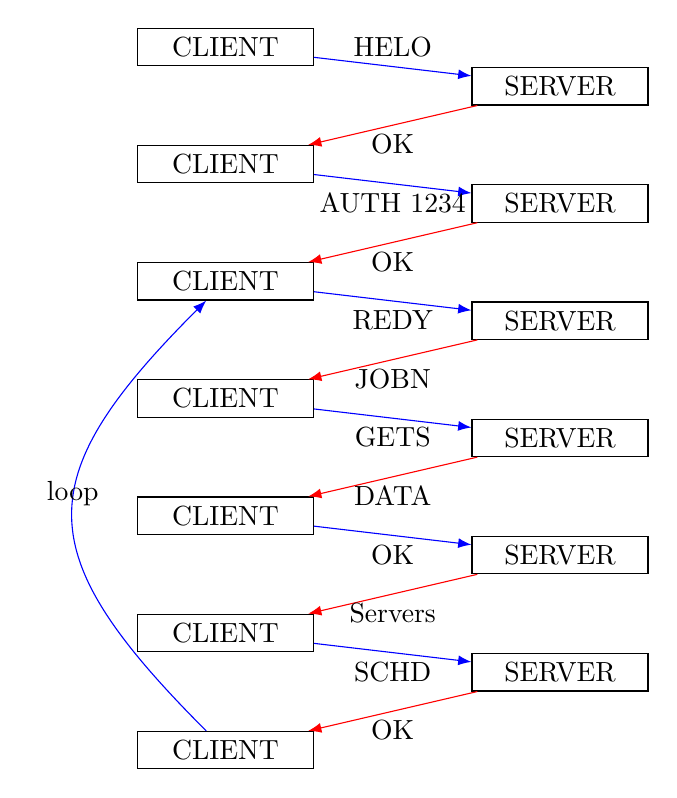
\begin{tikzpicture}[node distance=2cm,>=Latex]
        % Nodes
        \node (c1) [draw, text width=2cm, align=center] {CLIENT};
        \node (c2) [draw, below=1cm of c1, text width=2cm, align=center] {CLIENT};
        \node (c3) [draw, below=1cm of c2, text width=2cm, align=center] {CLIENT};
        \node (c4) [draw, below=1cm of c3, text width=2cm, align=center] {CLIENT};
        \node (c5) [draw, below=1cm of c4, text width=2cm, align=center] {CLIENT};
        \node (c6) [draw, below=1cm of c5, text width=2cm, align=center] {CLIENT};
        \node (c7) [draw, below=1cm of c6, text width=2cm, align=center] {CLIENT};

        \node (s1) [draw, right=of c1, yshift=-0.5cm, text width=2cm, align=center] {SERVER};
        \node (s2) [draw, below=1cm of s1, text width=2cm, align=center] {SERVER};
        \node (s3) [draw, below=1cm of s2, text width=2cm, align=center] {SERVER};
        \node (s4) [draw, below=1cm of s3, text width=2cm, align=center] {SERVER};
        \node (s5) [draw, below=1cm of s4, text width=2cm, align=center] {SERVER};
        \node (s6) [draw, below=1cm of s5, text width=2cm, align=center] {SERVER};

        % Arrows
        \draw[->, draw=blue] (c1) -- node[midway, above] {HELO} (s1);
        \draw[<-, draw=red] (c2) -- node[midway, below] {OK} (s1);
        \draw[->, draw=blue] (c2) -- node[midway, below] {AUTH 1234} (s2);
        \draw[<-, draw=red] (c3) -- node[midway, below] {OK} (s2);
        \draw[->, draw=blue] (c3) -- node[midway, below] {REDY} (s3);
        \draw[<-, draw=red] (c4) -- node[midway, below] {JOBN} (s3);
        \draw[->, draw=blue] (c4) -- node[midway, below] {GETS} (s4);
        \draw[<-, draw=red] (c5) -- node[midway, below] {DATA} (s4);
        \draw[->, draw=blue] (c5) -- node[midway, below] {OK} (s5);
        \draw[<-, draw=red] (c6) -- node[midway, below] {Servers} (s5);
        \draw[->, draw=blue] (c6) -- node[midway, below] {SCHD} (s6);
        \draw[<-, draw=red] (c7) -- node[midway, below] {OK} (s6);
        \draw[->, draw=blue] (c7) to[out=135, in=225, looseness=1.5] node[midway, above]{loop} (c3);

    \end{tikzpicture}
    \caption{Overview of GreetClient to DS-SIM flow}
    \label{fig:communication}
\end{figure}

\newpage

\section{Design}
% 3. Design (1 page): design philosophy, considerations and constraints, functionalities of each simulator component focusing on the client-side simulator

\subsection{Philosophy}
The design philosophy for the client-side simulator is centered around modularity, simplicity, and extensibility \cite{6654207}. The goal is to create a robust and flexible simulation environment that can easily adapt to varying requirements and scenarios. Key principles include modularity, where each component of the simulator is designed as an independent module, allowing for easy updates, maintenance, and testing \cite{7463700}. This is achieved through the separation of functional components AUTH and PROCESS in order to maintain a modular code base. Simplicity is also crucial, as the architecture and codebase are kept as straightforward as possible to ensure readability and ease of understanding for future developers, this extends into a culture of detailed documentation throughout the project. \cite{9711975} Lastly, extensibility is emphasized to ensure the system can accommodate new features and functionalities with minimal changes to existing components which can be seen in FC logic whereby there is room to expand into further algorithms.

In terms of constraints and considerations, a few key details are addressed. This includes functionality and performance which is addressed by utilising Macquarie ASH servers to perform tests as appose to local infrastructure. This off-site approach removes the limitations of using personal devices as the infrastructure contains the necessary components required to perform the operations of DS-SIM and GreetClient.

Further to this, Reliability and usability is also key. Macquarie university ASH servers are maintained and scaled by Macquarie and are assumed to be reliable in terms of performance, latency and compatibility, ensuring accuracy and consistency of simulation results. With regards to usability, the user interface and interaction mechanisms must be implemented in a way to be user-friendly. This was achieved through Visual Studio Code remote host connection whereby the developer in this case was familiar with the layout and controls of the application despite being used across locations. This ensured that the application was both usable and accessible at any given time. Finally, It's important to highlight network considerations as a factor in the philosophy of development both at ASH server side and Locally, ensuring that regular code changes are committed to Github and ASH servers are available requires a stable network connection.


GreetClient at first was designed to handle the input and output data for the simulation, processing user inputs, sending commands to the server, and handling server responses. However after rounds of review, it was determined that GreetClient serves to be run via script without necessary Input and output from User, no user interface and no scale able requirements outside of meeting the script objectives. Therefore a design shift was decided to move away from component based parsers, error handlers and other user based interactive components and more into smooth functional components in preparation for automation. Design decisions around GreetClient kept the focus around being optimised for quick data processing and minimal latency by removing as many debug statements and unecessary components as possible


Another key consideration involves the logging capabilities of the GreetClient along with the error handling process. Effective logging is crucial for maintaining a reliable and debuggable system. Logs should be detailed enough to assist in debugging and troubleshooting, capturing essential information such as timestamps, event types, and relevant data points. This level of detail allows developers to trace the sequence of events leading up to an issue, making it easier to identify and resolve bugs. Although this particular implementation does not consider detailed logging capabilities, the initial design had this in place.

In addition to logging, detailed and intuitive error handling is necessary to ensure the simulator remains user-friendly and resilient. Error messages should be clear and informative, providing users with enough context to understand what went wrong and how to address it. This includes specifying the nature of the error, potential causes, and possible solutions or workarounds. User-friendly error handling also involves gracefully managing exceptions, ensuring that the simulator can recover from errors without crashing or losing data.

\subsection{DS-SIM Principles} 
The initial design for the project required an understanding of the ds-sim relationship with the client application. Scoping out and understanding each message between the client and server was critical to understanding and interpreting the application. The requirement was for a First Capable implementation of the ds-client written in our own words, and if possible to improve on this implementation

\subsection{Algorithm Architecture}
\subsubsection{First Capable}
At a high level, First Capable simply selects the first capable server that appears after requesting a server list. This results in a fairly resource intensive operation as in many cases, the server that performs the job may be over equipped in terms of memory, cpu and storage. First capable does not consider ready jobs, waiting jobs which makes it a potential crutch in large scale operations whereby the logic in server selection fails to take into account these considerations.The design principle of first Capable is outlined under implementation but at a high level, it essentially selects the first server capable of performing the job after the server list is given to the client.

\subsubsection{Out performing Algorithm considerations}
Although not implemented in this project, a range of alternative algorithms were tested in order to achieve innovation marks. The design aspects of these algorithms relied on the components presented, including memory, cpu, disk, state, waiting jobs and ready jobs. Considerations in this space involved worst fit scenario, whereby the server with the lowest spec was selected to perform the job, Best fit whereby the best server was selected for the job and a mixture of waiting job list logic. Finally, a rating system was tested in which each server is given a value based on a set of criteria. 


\section{Implementation}
% 4. Implementation (2 pages): brief description of any implementation specific information including technologies, techniques, software libraries and data structures used. How each of components/functions of your simulator is implemented


\subsection{workshops}The project was implemented in a few stages determined by the tutorial workshops


\subsection{deliverables} For the assignment, implementation was based on a few key steps broken down into deliverables which were outlined in the README section of a repository. The code was maintained and stored in Github with some simple commit history and a few pull requests. The layout of the overall project can be seen below:

\begin{lstlisting}
/** "How's it tracking mate?"

    [x] Basic implementation (during tutorials)
    [x] set standard for docstring & linting of project
    [x]: Understand what FC implementation looks like
    [x]: Diagram & Pseudo FC
    [x]: Implement FC
    [x]: Linting & formatting
    [x]: Project documentation (LaTEX Template)
 */
\end{lstlisting}

\subsection{Specific components of GreetClient}
\subsubsection{Establish an initial connection the DS-SIM}
The initial connection DS-SIM is handled by the function setupConnection which is detailed below:

\begin{lstlisting}
/**
    Sets up connection and authentication with the server.

    Client sends HELO, receives OK
    Client sends AUTH, receives OK
     
    @param out PrintWriter for sending messages to the server
    @param in  BufferedReader for receiving messages from the server
    @throws IOException if an I/O error occurs while communicating with the server
*/

    private static void setupConnection(PrintWriter out, BufferedReader in) throws IOException {
  
        String msg = "HELO";
        String response;
        String auth = "SYSTEM";

        // HELO
        out.println(msg);
        if (!"OK".equals(in.readLine())){
            throw new IOException("HELO failed, Are you using correct DS-SIM?");
        }

        // AUTH
        msg = "AUTH " + auth;
        out.println(msg);
        if (!"OK".equals(in.readLine())){
            throw new IOException("AUTH failed, Are you using correct DS-SIM?");
        }
    }
\end{lstlisting}
This function meeds the initial requirement of GreetClient by establishing a connection to DS-SIM. It uses PrintWriter to handle writing output to a stream, BufferedReader to read text from an input stream and throws an input / output exception incase of any interruptions to this stream. From here, it follows the standard DS-SIM handshake method as follows:

\begin{figure}[h]
    \centering
    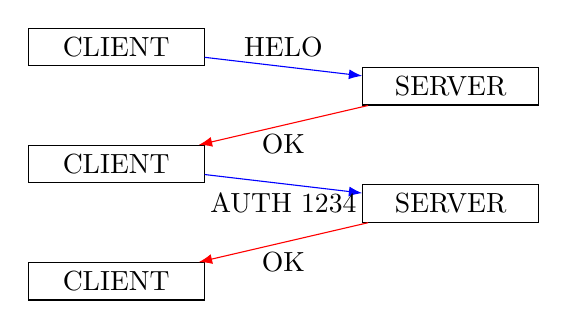
\begin{tikzpicture}[node distance=2cm,>=Latex]
        % Nodes
        \node (c1) [draw, text width=2cm, align=center] {CLIENT};
        \node (s1) [draw, right=of c1,yshift=-0.5cm, text width=2cm, align=center] {SERVER};
        \node (c2) [draw, below=1cm of c1, text width=2cm, align=center] {CLIENT};
        \node (s2) [draw, right=of c2,yshift=-0.5cm, text width=2cm, align=center] {SERVER};
        \node (c3) [draw, below=1cm of c2, text width=2cm, align=center] {CLIENT};

        % Arrows
        \draw[->, draw=blue] (c1) -- node[midway, above] {HELO} (s1);
        \draw[<-, draw=red] (c2) -- node[midway, below] {OK} (s1);
        \draw[->, draw=blue] (c2) -- node[midway, below] {AUTH 1234} (s2);
        \draw[<-, draw=red] (c3) -- node[midway, below] {OK} (s2);

    \end{tikzpicture}
    \caption{Establish an initial connection the DS-SIM}
    \label{fig:communication}
\end{figure}

\subsubsection{Ingest job and server information}
At this stage, the client is Authenticated and is ready to begin the main loop in order to request and schedule all jobs available. This is defined in ProcessJobInfo which takes the IN/OUT param similar to above and will throw an I/O error if communication is disrupted. 
\begin{lstlisting}
    /**
     * Processes job information received from the server.
     *
     * @param out PrintWriter for sending messages to the server
     * @param in  BufferedReader for receiving messages from the server
     * @throws IOException if an I/O error occurs while communicating with the server
     */
\end{lstlisting}

An important part of this loop is the ability to handle NONE and JCPL responses from the server. A none response essentially tells Client that there are no more jobs, at which point the client responds with QUIT to kill the connection. If the server sends a JCPL, this indicates that a job has been completed and this information is added to a list. Early versions would print this list at the end of a loop for debugging however in the finalized version, this is not necessary however the JCPL info is still stored.

\begin{lstlisting}

     .....
     // Handle NONE response
    if ("NONE".equals(response)) {
        out.println("QUIT");
    ....
    // Handle JCPL response
    if (response.contains("JCPL")) {
        jcplList.add(response);
        continue;
\end{lstlisting}

Another important feature within this function is the ability to split and sort information received from the server. This is done by opening a String array and setting response.split after which each section of the array is declared based on it's functionality. For example, JobID is the expected return at index 1 of the list, therefore it's declared here for re-use later in a readable format.

\begin{lstlisting}
    // Split the received line by whitespace
    String[] jobParts = response.split("\\s+");
    ...
    // Assign each part to corresponding variables
    String jobType = jobParts[0];
    int jobID = Integer.parseInt(jobParts[1]);
    int core = Integer.parseInt(jobParts[3]);
    int memory = Integer.parseInt(jobParts[4]);
    int disk = Integer.parseInt(jobParts[5]);
\end{lstlisting}

After the information is split and parsed, Client sends a get request to the server. This is achieved by selecting the required information (Core, Memory and Disk) then sending a crafted response to the server

\begin{lstlisting}

    // 3. Send GETS to the server
    // e.g. GETS Capable <core> <memory> <disk>
    String getsRequest = "GETS " + "Capable" + " " + core + " " + memory + " " + disk;
    out.println(getsRequest);
\end{lstlisting}

The flow of this process can be seen below in Fig3:

\begin{figure}[h]
    \centering
    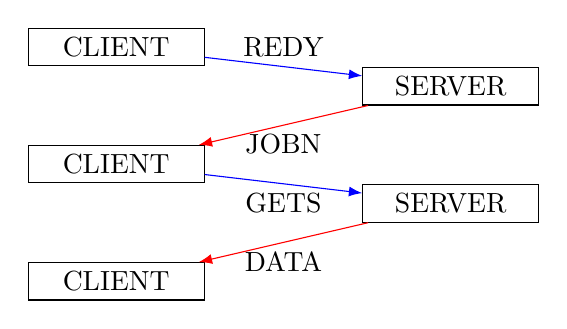
\begin{tikzpicture}[node distance=2cm,>=Latex]
        % Nodes
        \node (c1) [draw, text width=2cm, align=center] {CLIENT};
        \node (s1) [draw, right=of c1,yshift=-0.5cm, text width=2cm, align=center] {SERVER};
        \node (c2) [draw, below=1cm of c1, text width=2cm, align=center] {CLIENT};
        \node (s2) [draw, right=of c2,yshift=-0.5cm, text width=2cm, align=center] {SERVER};
        \node (c3) [draw, below=1cm of c2, text width=2cm, align=center] {CLIENT};

        % Arrows
        \draw[->, draw=blue] (c1) -- node[midway, above] {REDY} (s1);
        \draw[<-, draw=red] (c2) -- node[midway, below] {JOBN} (s1);
        \draw[->, draw=blue] (c2) -- node[midway, below] {GETS} (s2);
        \draw[<-, draw=red] (c3) -- node[midway, below] {DATA} (s2);

    \end{tikzpicture}
    \caption{Ingest job and server information}
    \label{fig:communication}
\end{figure}

\subsubsection{Distribute the jobs across DS-SIM}
This phase of the program determines which server receives which job and consists of a response parse split followed by a selectBestServer function. The main highlight here is the split of server information based on selectBestServer whereby each component of the response is ingested and analysed. At this point, the implementation is carefully considered as to how to respond to the server with the correct selection in a SCHD command. This is essentially the core functionality of the Client app and the implementation shown below is for First Capable. 

\begin{lstlisting}
    /**
     * Selects the best server based on the given criteria.
     *
     * @param servers List of server information arrays where each array contains server details
     * @param jobCore Number of cores required by the job
     * @param jobMemory Amount of memory required by the job
     * @param jobDisk Amount of disk space required by the job
     * @return An array containing the details of the selected server or null if no suitable server is found
     */
\end{lstlisting}

At this stage, the list of servers is sent to the client and the client is required to handle the response including white spaces and line splits. This is achieved through a List String array which populates all of the information received from the server. numLines counts the lines given and then for each line in numLines, the servers are sorted into a list of arrays.
\begin{lstlisting}
    // 6. Receive and organize server data
    List<String[]> servers = new ArrayList<>();
    for (int i = 0; i < numLines; i++) {
        String line = in.readLine().trim();
        servers.add(line.split("\\s+"));
    }
\end{lstlisting}

The selectBestServer function provides the functionality to choose a server with the information provided in the servers array list. For each item, at this point the client is able to select different parameters of the server such as core, cpu, ram, state, waiting jobs or ready jobs to determine which server should be selected in order to run this particular job. There have been several implementation attempts at this function however the implementation below servers to demonstrate First Capable, whereby the first server from the list is chosen. 
\begin{lstlisting}
    /**
     * Selects the best server based on the given criteria.
     *
     * @param servers List of server information arrays where each array contains server details
     * @param jobCore Number of cores required by the job
     * @param jobMemory Amount of memory required by the job
     * @param jobDisk Amount of disk space required by the job
     * @return An array containing the details of the selected server or null if no suitable server is found
     */
    private static String[] selectBestServer(List<String[]> servers, int jobCore, int jobMemory, int jobDisk) {
    String[] bestServer = null;
    if (!servers.isEmpty()) {
        bestServer = servers.get(0); // First Capable logic
    }
    return bestServer;
    }
\end{lstlisting}

selectBestServer is called based on bestServer which is then used in the following section to schedule the job. As long as a server was selected, the SCHD message is created and sent to the server which is the final stage of the overarching loop. At this point, the SCHD message is sent to DS-SIM, the job is scheduled and the loop returns to wait for a further response from DS-IM.
\begin{lstlisting}

    // 7. Select the bset server based on criteria
    String[] bestServer = selectBestServer(servers, core, memory, disk);

    //8. Schedule job to the best server
    if (bestServer != null){
        String serverType = bestServer[0];
        String serverID = bestServer[1];
        String schdMsg = "SCHD" + " " + jobID + " " + serverType + " " + serverID;
        out.println(schdMsg);
        in.readLine(); // Read the response
    }
\end{lstlisting}

The above server selection and scheduling parts can be summarised in the below fig4 which outlines the client and server communication for this final stage. After this point, the Client loops back into REDY to receive a further job from DS-SIM and will function as intended until NONE is received or an invalid response is detected.

\begin{figure}[h]
    \centering
    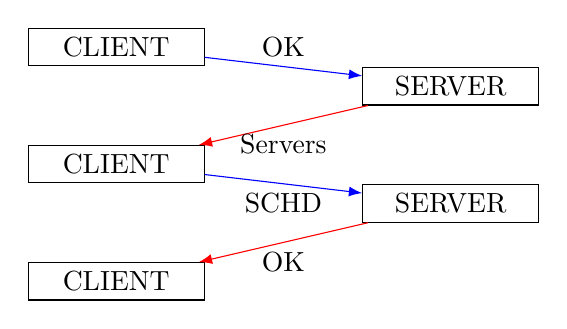
\begin{tikzpicture}[node distance=2cm,>=Latex]
        % Nodes
        \node (c1) [draw, text width=2cm, align=center] {CLIENT};
        \node (s1) [draw, right=of c1,yshift=-0.5cm, text width=2cm, align=center] {SERVER};
        \node (c2) [draw, below=1cm of c1, text width=2cm, align=center] {CLIENT};
        \node (s2) [draw, right=of c2,yshift=-0.5cm, text width=2cm, align=center] {SERVER};
        \node (c3) [draw, below=1cm of c2, text width=2cm, align=center] {CLIENT};

        % Arrows
        \draw[->, draw=blue] (c1) -- node[midway, above] {OK} (s1);
        \draw[<-, draw=red] (c2) -- node[midway, below] {Servers} (s1);
        \draw[->, draw=blue] (c2) -- node[midway, below] {SCHD} (s2);
        \draw[<-, draw=red] (c3) -- node[midway, below] {OK} (s2);

    \end{tikzpicture}
    \caption{Distribute the jobs across DS-SIM}
    \label{fig:communication}
\end{figure}


\section{References}
Github link:  \href{https://github.com/MQU-COMP3100/comp3100-assignment-2-Ajsensai?tab=readme-ov-file}{github link}

(https://github.com/MQU-COMP3100/comp3100-assignment-2-Ajsensai?tab=readme-ov-file)

Thankyou to our Tutor Jaden for his insight and support throughout this project

\bibliography{references}{}
\bibliographystyle{IEEEtran}

\end{document}
